\section{Calculation of Renyi entropy}
\begin{itemize}
\item
Now we calculate the Renyi entropy for the state $\rho$ from \eqref{rhomatrix} for an arbitrary parameter $\alpha$. The calculation process stays the same as in the case of the vonNeumann entropy, up until the function implementation at \eqref{functionimp} in which we change the function $F$ to the function $r$ adapted to \defref{renyi}:
\begin{align}
\label{functionimp1}
R(\alpha;\rho) &= \frac{1}{1-\alpha}\log \left\{ \Tr \left[ r(\alpha;\rho) \right] \right\} \\[0.5em]
&= \frac{1}{1-\alpha}\log \left\{ \Tr \left[ r(\alpha;MDM^{-1}) \right] \right\} \\[0.5em]
&=\frac{1}{1-\alpha} \log \left\{ \Tr \left[
M
\left( \begin{array}{cccc}
 1^{\alpha} & 0 & 0 & 0 \\
 0 & 0^{\alpha} & 0 & 0 \\
 0 & 0 & 0^{\alpha} & 0 \\
 0 & 0 & 0 & 0^{\alpha} \\
\end{array}
\right)
M^{-1}
\right]
\right\}
\nonumber\\[0.5em]
&=\frac{1}{1-\alpha} \log \left[ \frac{1}{2}\Tr \left(
\begin{array}{cccc}
 0 & 0 & 0 & 0 \\
 0 & 1 & i & 0 \\
 0 & -i & 1 & 0 \\
 0 & 0 & 0 & 0 \\
\end{array}
\right)
\right] \\[0.5em]
&=0
\end{align}

This is of course expected since the Renyi entropy has a minimum value of $0$ iff $\rho$ is a pure state. 
\item
Let's calculate the Renyi entropy of the diagonal density matrix $\rho$ in \eqref{ffrefer} using both $0<s<1$ and $\alpha \in(0,1) \cup(1, \infty)$ as free parameters:
\begin{align}
R(\alpha;\rho(s)) 
&= \frac{1}{1-\alpha} \log \left \{ \Tr \left[ r(\alpha;\rho(s)) \right] \right\} \\[0.5em]
&= \frac{1}{1-\alpha} \log \left\{  \Tr \left[ \left(
\begin{array}{cc}
 r(\alpha;s) & 0 \\
 0 & r(\alpha;1-s) \\[0.5em]
\end{array}
\right) \right] \right\}\\[0.5em]
&=
\frac{1}{1-\alpha} \log \left\{  \Tr \left[ \left(
\begin{array}{cc}
 s^{\alpha} & 0 \\
 0 & (1-s)^{\alpha} \\[0.5em]
\end{array}
\right) \right] \right\} \\[0.5em] 
&=\frac{1}{1-\alpha}
\log \left[ s^{\alpha }+(1-s)^{\alpha } \right]
\end{align}
Let's plot for different values of $\alpha$:
\begin{figure}[H]
\label{figure3}
\begin{center}
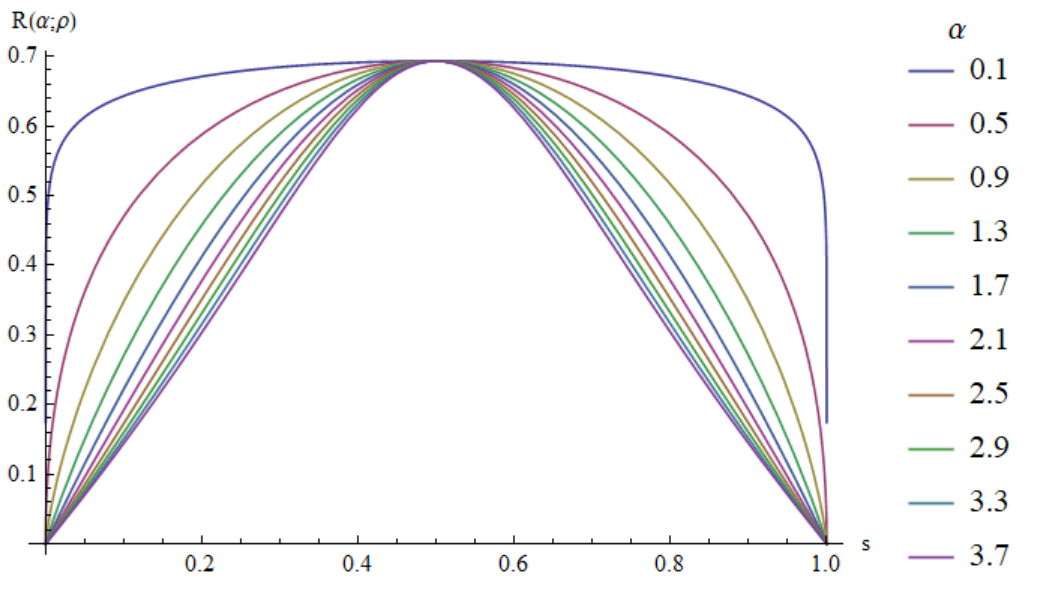
\includegraphics[scale=0.8]{figures/renyi_ent_plot.png}
\caption{Two points to make: (a)$\lim_{\alpha \to 1}R(\alpha,\rho) = S(\rho)$ is demonstrated via the similarities with figure \ref{figure1}, (b) for $s=0.5$ Renyi entropy takes the value $\log2$ independent of $\alpha$.}
\end{center}
\end{figure}
and in $3D$ for more intuition:
\begin{figure}[H]
\begin{center}
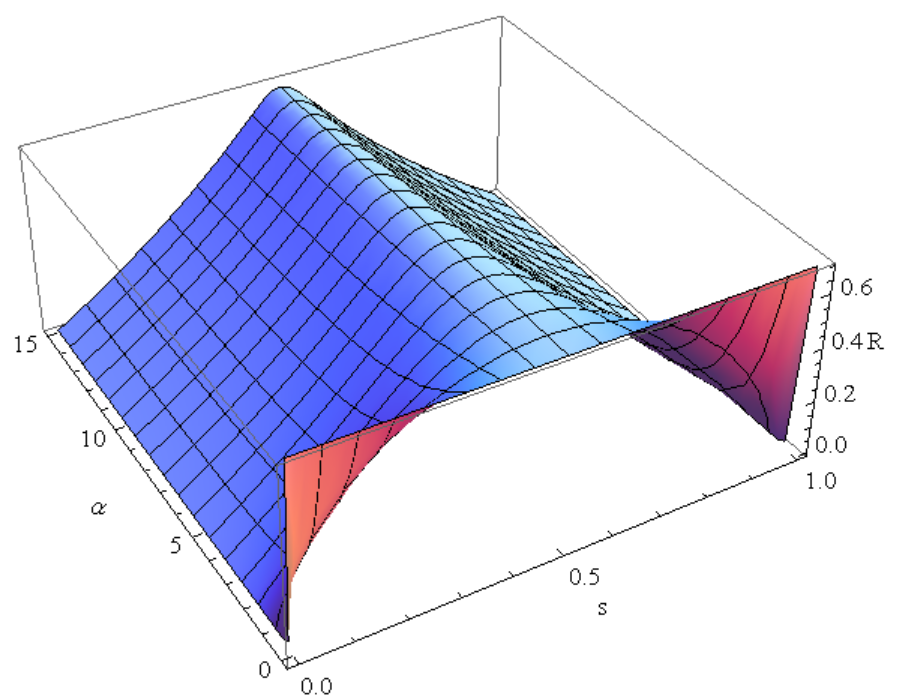
\includegraphics[scale=0.7]{figures/renyi_ent_plot_3D.png}
\caption{The 3-D plot based on the two parameters $s$ and $\alpha$.}
\label{figuridion3d}
\end{center}
\end{figure}
Regarding the example \eqref{asdasdas} the Renyi entropy is: 
\begin{align}
R(\alpha;\rho) &= \frac{1}{1-a} \log \left\{ \Tr \left[ \diag \big( r(\alpha;\rho_{0}),r(a;\rho_{1}),..,r(a;\rho_{N-2}),r(a; \rho_{N-1})
 \big) \right] \right\} \\[0.5 em] 
 &=\frac{1}{1-a} \log \left( \sum_{i=0}^{N-1}\rho_{i}^{\alpha} \right)
\end{align}
For the special case that $\rho_{i}=1/N$ we can easily see that:
\begin{equation}
R(\alpha;\rho)=\log N
\end{equation}
independent of $\alpha$.
\end{itemize}